\documentclass[a4paper,12pt]{report}

% Page layout
\usepackage[left=2.5cm,right=2.5cm,top=2.5cm,bottom=2.5cm]{geometry}

% Font and text
\usepackage[afrikaans,english]{babel}
\usepackage{microtype}
\usepackage{setspace}
\usepackage{lmodern}
\usepackage{siunitx}
\newcommand{\myemph}[1]{{\sffamily\bfseries#1}}
\sloppy
\onehalfspacing

% Headings
\usepackage[raggedright,sf,bf]{titlesec}
\usepackage[margin=\the\parindent,small,bf,sf]{caption}
\titlelabel{\thetitle.\ }
\titleformat{\chapter}[display]{\huge\bfseries\sffamily}{\chaptertitlename\ \thechapter}{15pt}{\Huge \raggedright}
\titlespacing*{\chapter}{0pt}{0pt}{40pt}  % remove spacing before chapter headings
\makeatletter
\let\originall@chapter\l@chapter
\def\l@chapter#1#2{\originall@chapter{{\sffamily #1}}{#2}}
\makeatother

%% Alternative headings using small-caps (comment out the top section)
%\usepackage[raggedright,bf]{titlesec}
%\usepackage[margin=\the\parindent,small,bf]{caption}
%\titlelabel{\thetitle.\ }
%\titleformat{\chapter}[display]{\huge\scshape}{\chaptertitlename\ \thechapter}{15pt}{\Huge \raggedright}
%\titlespacing*{\chapter}{0pt}{0pt}{40pt}  % remove spacing before chapter headings

% Table of contents
\let \savenumberline \numberline
\def \numberline#1{\savenumberline{#1.}}

% Figures
\usepackage{graphicx}
\usepackage{pdfpages}
\usepackage{subcaption}
\setlength{\abovecaptionskip}{7.5pt}  % spacing above and below captions
\newcommand*{\WaterMark}[2][0.2\paperwidth]{\AddToShipoutPicture*{\AtTextCenter{\parbox[c]{0pt}{\makebox[0pt][c]{\includegraphics[width=#1]{#2}}}}}}

% Mathematics
\usepackage[cmex10]{amsmath}
\usepackage{amssymb}
\usepackage{cancel}
\DeclareMathOperator*{\argmax}{arg\,max}
\newcommand{\T}{^\top}
\newcommand{\tr}{\textrm{tr}}
\renewcommand{\vec}[1]{\boldsymbol{\mathbf{#1}}}
\newcommand{\defeq}{\triangleq}

% Tables
\usepackage{booktabs}
\usepackage{tabularx}
\usepackage{multirow}
\newcommand{\mytable}{
    \centering
    \small
    \renewcommand{\arraystretch}{1.2}
    }
\renewcommand{\tabularxcolumn}[1]{m{#1}}
\newcolumntype{C}{>{\centering\arraybackslash}X}
\newcolumntype{L}{>{\raggedright\arraybackslash}X}
\usepackage{tablefootnote}

% Header and footer
\usepackage{fancyhdr}
\pagestyle{fancy}
\fancyhf{}
\renewcommand{\sectionmark}[1]{\markright{\normalsize \thesection.\ #1}}
\fancyhead[C]{\nouppercase{\textit{\rightmark}}}
\fancyhead[RO]{\thepage}
 \fancyhead[LE]{\thepage}  % double-sided printing
\fancyfoot{}
\setlength\headheight{14.5pt}
\renewcommand{\headrulewidth}{0pt}
\fancypagestyle{plain}{\fancyhead{}
                       \renewcommand{\headrulewidth}{0pt}
                       \fancyfoot[C]{\thepage}}

% Pseudo-code
\usepackage{algorithm}  % should go before \usepackage{hyperref}

% Table of contents and hyperlinks
\usepackage{hyperref}
\hypersetup{colorlinks=true,linktoc=all,citecolor=black,linkcolor=black}
\usepackage[nottoc]{tocbibind}

% Pseudo-code
\usepackage{algpseudocode}  % should go after \usepackage{hyperref}
\renewcommand{\thealgorithm}{\arabic{chapter}.\arabic{algorithm}} 
\captionsetup[algorithm]{labelfont={bf,sf},font=small,labelsep=colon}

% Bibliography
\usepackage{cite}  % automatically reorder inline citations
\bibliographystyle{IEEEtran}

% Fix titlesec issue
\usepackage{etoolbox}
\makeatletter
\patchcmd{\ttlh@hang}{\parindent\z@}{\parindent\z@\leavevmode}{}{}
\patchcmd{\ttlh@hang}{\noindent}{}{}{}
\makeatother

% Own
% Acronyms
\usepackage{acronym}


\begin{document}

% Front matter
\graphicspath{{frontmatter/fig/}}
\pagenumbering{Alph}

\begin{titlepage}
	\begin{center}
		
		
\includegraphics[width=10cm]{USlogo-top}
		
		\vfill
		
		{\sffamily \bfseries \huge A Critical Analysis of Design Flaws in the Death Star \par}
%		{\scshape \huge A Critical Analysis of Design Flaws in the Death Star \par}
		
		\vfill
		
		{\large {\Large Gabrielle Liebenberg} \\ 22546723 \par}
		
		\vfill
		
		\vfill
		
		{Report submitted in partial fulfilment of the requirements of the module \\
			Project (E) 448 for the degree Baccalaureus in Engineering in the Department of
			Electrical and Electronic Engineering at Stellenbosch University. \par}
		
		\vfill
		
		{\large {Supervisor}: Dr O.\ W.\ Kenobi} %\\
		% Department of Electrical and Electronic Engineering \par}
		
		\vfill
		
		{\Large June 2024}
	\end{center}
\end{titlepage}

%\graphicspath{{frontmatter/fig/}}
\pagenumbering{Alph}

\begin{titlepage}
	\begin{center}
		
		%
\includegraphics[width=10cm]{USlogo-top}
		
		\WaterMark{UScrest-WM}
		
		~\vspace{4.5em}
		
		{\sffamily \bfseries \huge A Critical Analysis of Design Flaws in the Death Star \par}
%		{\scshape \huge A Critical Analysis of Design Flaws in the Death Star \par}		
		
		\vspace{7em}
		
		{\large {\Large  Luke Skywalker} \\ 99652154 \par}
		
		\vspace{8em}
		
		{\large Thesis presented in partial fulfilment of the requirements for the degree of \\ Master of Engineering (Electronic) in the Faculty of Engineering at Stellenbosch University. \par}
		
		\vfill
		
		{\large {Supervisor}: Dr O.\ W.\ Kenobi\\
		Department of Electrical and Electronic Engineering \par}
		
		%\vfill
		\vspace{10em}
		
		{\Large October 2099}
	\end{center}
\end{titlepage}

\pagenumbering{roman}
\chapter*{Acknowledgements}
% \addcontentsline{toc}{chapter}{Acknowledgements}
\makeatletter\@mkboth{}{Acknowledgements}\makeatother

I would like to thank my dog, Muffin. I also would like to thank the inventor of the incubator; without him/her, I would not be here. Finally, I would like to thank Dr Herman Kamper for this amazing report template.

%\chapter*{Declaration}
\newpage
\thispagestyle{plain}
\addcontentsline{toc}{chapter}{Declaration}
\makeatletter\@mkboth{}{Declaration}\makeatother

\centerline{
\includegraphics[width=8cm]{USlogo-top}}
\vspace*{-10pt}

\section*{\centering Plagiaatverklaring / \textit{Plagiarism Declaration}}

\vspace*{5pt}

\begin{enumerate}
    \item Plagiaat is die oorneem en gebruik van die idees, materiaal en ander intellektuele eiendom van ander persone asof dit jou eie werk is.\\
    \textit{Plagiarism is the use of ideas, material and other intellectual property of another's work
        and to present is as my own.}
    
    \item Ek erken dat die pleeg van plagiaat 'n strafbare oortreding is aangesien dit 'n vorm van diefstal is.\\
    \textit{I agree that plagiarism is a punishable offence because it constitutes theft.}
    
    \item Ek verstaan ook dat direkte vertalings plagiaat is. \\
    \textit{I also understand that direct translations are plagiarism.}
    
    \item Dienooreenkomstig is alle aanhalings en bydraes vanuit enige bron (ingesluit die internet) volledig verwys (erken). Ek erken dat die woordelikse aanhaal van teks sonder aanhalingstekens (selfs al word die bron volledig erken) plagiaat is. \\
    \textit{Accordingly all quotations and contributions from any source whatsoever (including the internet) have been cited fully. I understand that the reproduction of text without quotation marks (even when the source is cited) is plagiarism}
    
    \item Ek verklaar dat die werk in hierdie skryfstuk vervat, behalwe waar anders aangedui, my eie oorspronklike werk is en dat ek dit nie vantevore in die geheel of gedeeltelik ingehandig het vir bepunting in hierdie module/werkstuk of 'n ander module/werkstuk~nie. \\
    \textit{I declare that the work contained in this assignment, except where otherwise stated, is my original work and that I have not previously (in its entirety or in part) submitted it for grading in this module/assignment or another module/assignment.}
\end{enumerate}

\vfill

\noindent \begin{tabularx}{1.0\linewidth}{|L|L|}
    \hline
    \vspace{1cm} {Studentenommer / \textit{Student number}} & \vspace{1cm} {Handtekening / \textit{Signature}} \\
    \hline
    \vspace{1cm} {Voorletters en van / \textit{Initials and surname}} & \vspace{1cm} {Datum / \textit{Date}} \\
    \hline
\end{tabularx}

\vspace{15pt}

% The old declaration

%I, the undersigned, hereby declare that the work contained in this report is my own original work unless otherwise stated.
%
%% Afrikaans:
%% Hiermee verklaar ek, die ondergetekende, dat die werk in hierdie verslag vervat my eie oorspronklike werk is, tensy anders vermeld.
%
%\vspace{2.5cm}
%
%\begin{table}[h]
%\begin{tabular}{@{}p{2.5cm}p{5cm}}
%    Signature: & \dotfill \\
%    & \multicolumn{1}{c}{Obi-Wan Kenobi} \\
%    ~\vspace{1cm} \\
%    Date: & \dotfill \\
%\end{tabular}
%\end{table}
%
%\vfill
%
%\begin{center}
%    Copyright \textcopyright\ 2099 Stellenbosch University \\
%    All rights reserved
%\end{center}


\chapter*{Abstract}
\addcontentsline{toc}{chapter}{Abstract}
\makeatletter\@mkboth{}{Abstract}\makeatother

\subsubsection*{English}

The English abstract.

\selectlanguage{afrikaans}

\subsubsection*{Afrikaans}

Die Afrikaanse uittreksel.

\selectlanguage{english}

\tableofcontents
\listoffigures
\listoftables
\chapter*{Nomenclature\markboth{}{Nomenclature}}
\addcontentsline{toc}{chapter}{Nomenclature}

% \vspace*{-3mm}
\subsubsection*{Variables and functions}

\begingroup
\renewcommand{\arraystretch}{1.2}
\renewcommand{\tabularxcolumn}[1]{p{#1}}
\begin{tabularx}{\textwidth}{@{}p{2.5cm}L}
    $p(x)$ & Probability density function with respect to variable $x$.\\
    $P(A)$ & Probability of event $A$ occurring.\\
    $\varepsilon$ & The Bayes error. \\
    $\varepsilon_u$ & The Bhattacharyya bound. \\
    $B$ & The Bhattacharyya distance. \\
    $s$ & An HMM state.  A subscript is used to refer to a particular state, e.g.\ $s_i$ refers to the $i^{\text{th}}$ state of an HMM. \\
    $\mathbf{S}$ & A set of HMM states. \\
    $\mathbf{F}$ & A set of frames. \\
    $\mathbf{o}_f$ & Observation (feature) vector associated with frame $f$. \\
    $\gamma_s(\mathbf{o}_f)$ & A posteriori probability of the observation vector $\mathbf{o}_f$ being generated by HMM state $s$. \\
    $\mu$ & Statistical mean vector. \\
    $\Sigma$ & Statistical covariance matrix. \\
    $L(\mathbf{S})$ & Log likelihood of the set of HMM states $\mathbf{S}$ generating the training set observation vectors assigned to the states in that set. \\
    $\mathcal{N}(\mathbf{x} | \mu, \Sigma)$ & Multivariate Gaussian PDF with mean $\mu$ and covariance matrix $\Sigma$.\\
    $a_{ij}$ & The probability of a transition from HMM state $s_i$ to state $s_j$. \\
    $N$ & Total number of frames or number of tokens, depending on the context. \\
    $D$ & Number of deletion errors. \\
    $I$ & Number of insertion errors. \\
    $S$ & Number of substitution errors. \\
\end{tabularx}
\endgroup


\newpage
\subsubsection*{Acronyms and abbreviations}

\begingroup
\renewcommand{\arraystretch}{1.2}
\begin{tabular}{@{}p{2.5cm} l}
    AE      & Afrikaans English \\
    AID     & accent identification \\
    ASR     & automatic speech recognition \\
    AST     & African Speech Technology \\
    CE      & Cape Flats English \\
    DCD     & dialect-context-dependent \\
    DNN		& deep neural network \\
    G2P     & grapheme-to-phoneme \\
    GMM     & Gaussian mixture model \\
    HMM     & hidden Markov model \\
    HTK     & Hidden Markov Model Toolkit \\
    IE      & Indian South African English \\
    IPA     & International Phonetic Alphabet \\
    LM      & language model \\
    LMS     & language model scaling factor \\
    MFCC    & Mel-frequency cepstral coefficient \\
    MLLR    & maximum likelihood linear regression \\
    OOV     & out-of-vocabulary \\
    PD      & pronunciation dictionary \\
    PDF     & probability density function \\
    SAE     & South African English \\
    SAMPA   & Speech Assessment Methods Phonetic Alphabet \\
\end{tabular}
\endgroup

\newpage
\pagenumbering{arabic}

% Contents
\graphicspath{{introduction/fig/}}

\chapter{Introduction}
\label{chap:introduction}

During the COVID-19 lockdown in 2020, gardening became a popular method of relieving stress \cite{covid_stress_study} and improving mental health and resilience \cite{mental_resiliance_study}. Additionally, gardening provides physical and psychological benefits to older adults \cite{seniors_psych_study}, many of whom have to adjust their gardening practices as they age and become unable to safely perform some tasks \cite{seniors_garden_study}.

Automating crucial tasks would allow individuals to start and maintain healthy, productive gardens despite the inability to reliably maintain them manually.
\\

This paper focuses specifically on indoor herb gardens as monitoring and maintaining larger outdoor gardens requires larger, more complex systems that would require significantly more time and resources to develop.
\\

Soil moisture levels have been shown to be an important factor in the distribution, growth and development of herbs, along with air humidity \cite{humidity_moisture_study}. Additionally, soil moisture levels influence the root/shoot ratio of herbs. Higher levels of soil moisture lead to a larger percentage of herb growth occurring above ground \cite{root_shoot_study}. In the case of herbs grown for cooking, this is ideal as it leads to more usable leaves. 
\\

A device that is able to automatically monitor and maintain optimal ground moisture levels will therefore provide the largest benefit to maintaining a healthy indoor herb garden.

\section{Project Objectives}
This project aims to design, build and test a device that will:
\begin{itemize}
    \item Monitor ground moisture levels
    \item Monitor exposure to sunlight
    \item Automatically water the soil to maintain optimal moisture levels
    \item Display recorded data and allow the user to adjust desired soil moisture levels using a mobile application
    \item Reliably function despite power outages
\end{itemize}


\graphicspath{{literature_study/fig/}}

\chapter{Literature Study}
\label{chap:literature_study}

\section{Soil moisture sensor}
Capacitive soil moisture sensors have two electrodes that form a planar capacitor with soil acting as the dielectric material as shown in figure \ref{fig:capacitor}. 

\begin{figure}[!h]
    \centering
    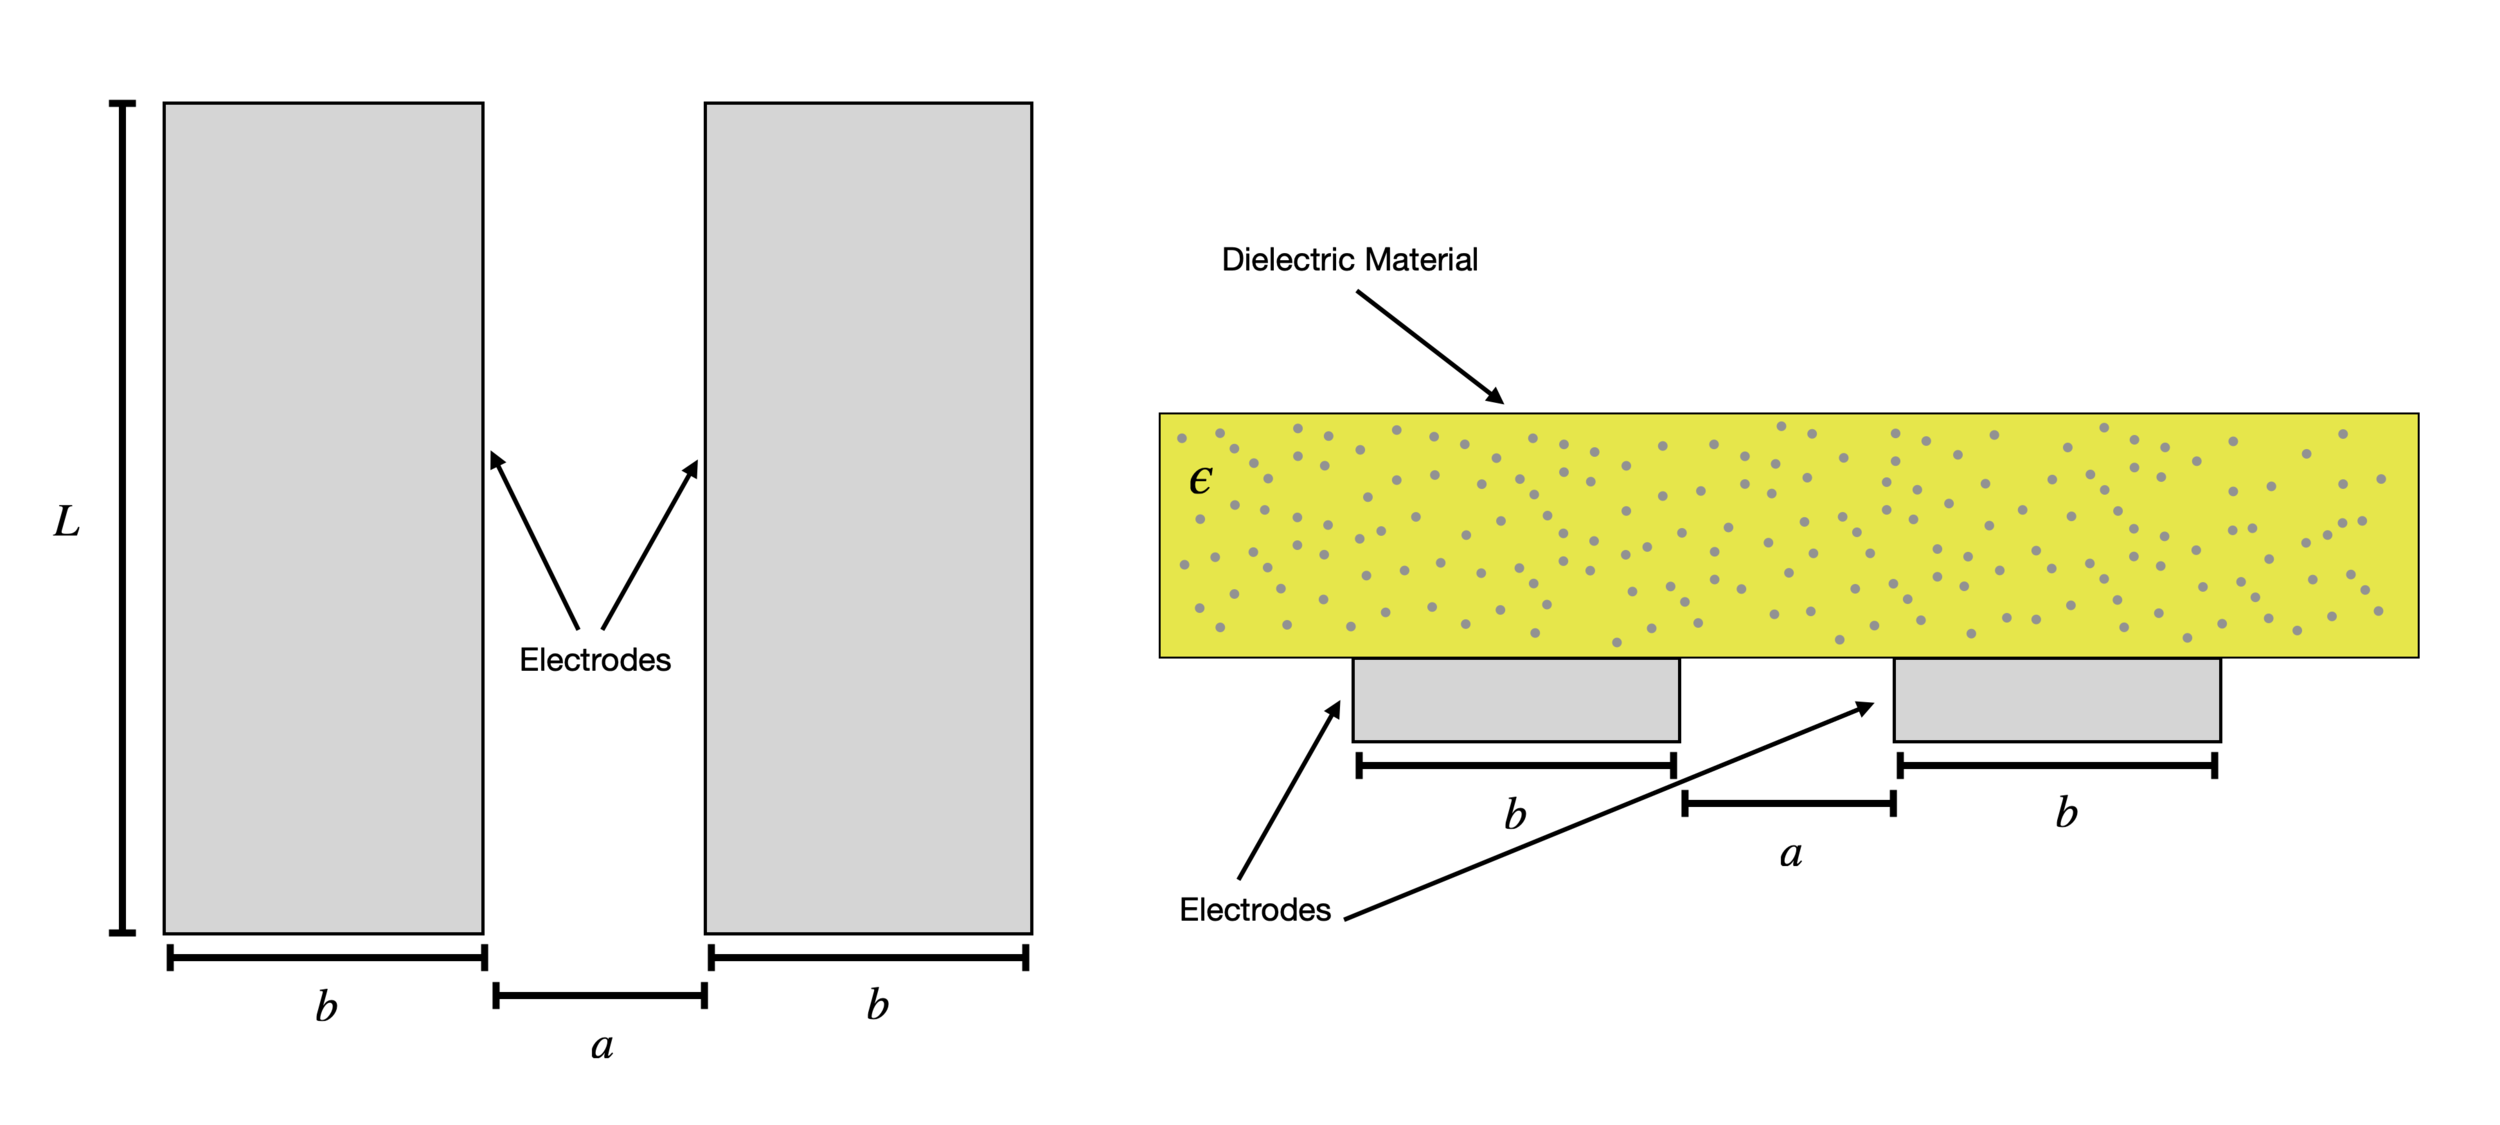
\includegraphics[width= 0.9\linewidth]{coplanar_capacitor_drawing.png}
    \caption{Planar capacitor \cite{moisture_sensor_img}}
    \label{fig:capacitor}
\end{figure}

The percentage of water will change the dielectric constant of the soil and therefore the capacitance. The sensor uses a timer to output a PWM voltage proportional to the capacitance of the soil. \cite{moisture_sensor_img}

\section{UV light sensor}
Ultraviolet light has a wavelength range of 100 to 400 nm and can be measured using a photodiode or photo-resistor. These produce either a current or resistance that is dependant on UV radiation. The sensor outputs a voltage proportional to this current or resistance. \cite{UV_sensor}
\graphicspath{{general_design/fig/}}

\chapter{Design}
\label{chap:general_design}

\begin{figure}[!h]
    \centering
    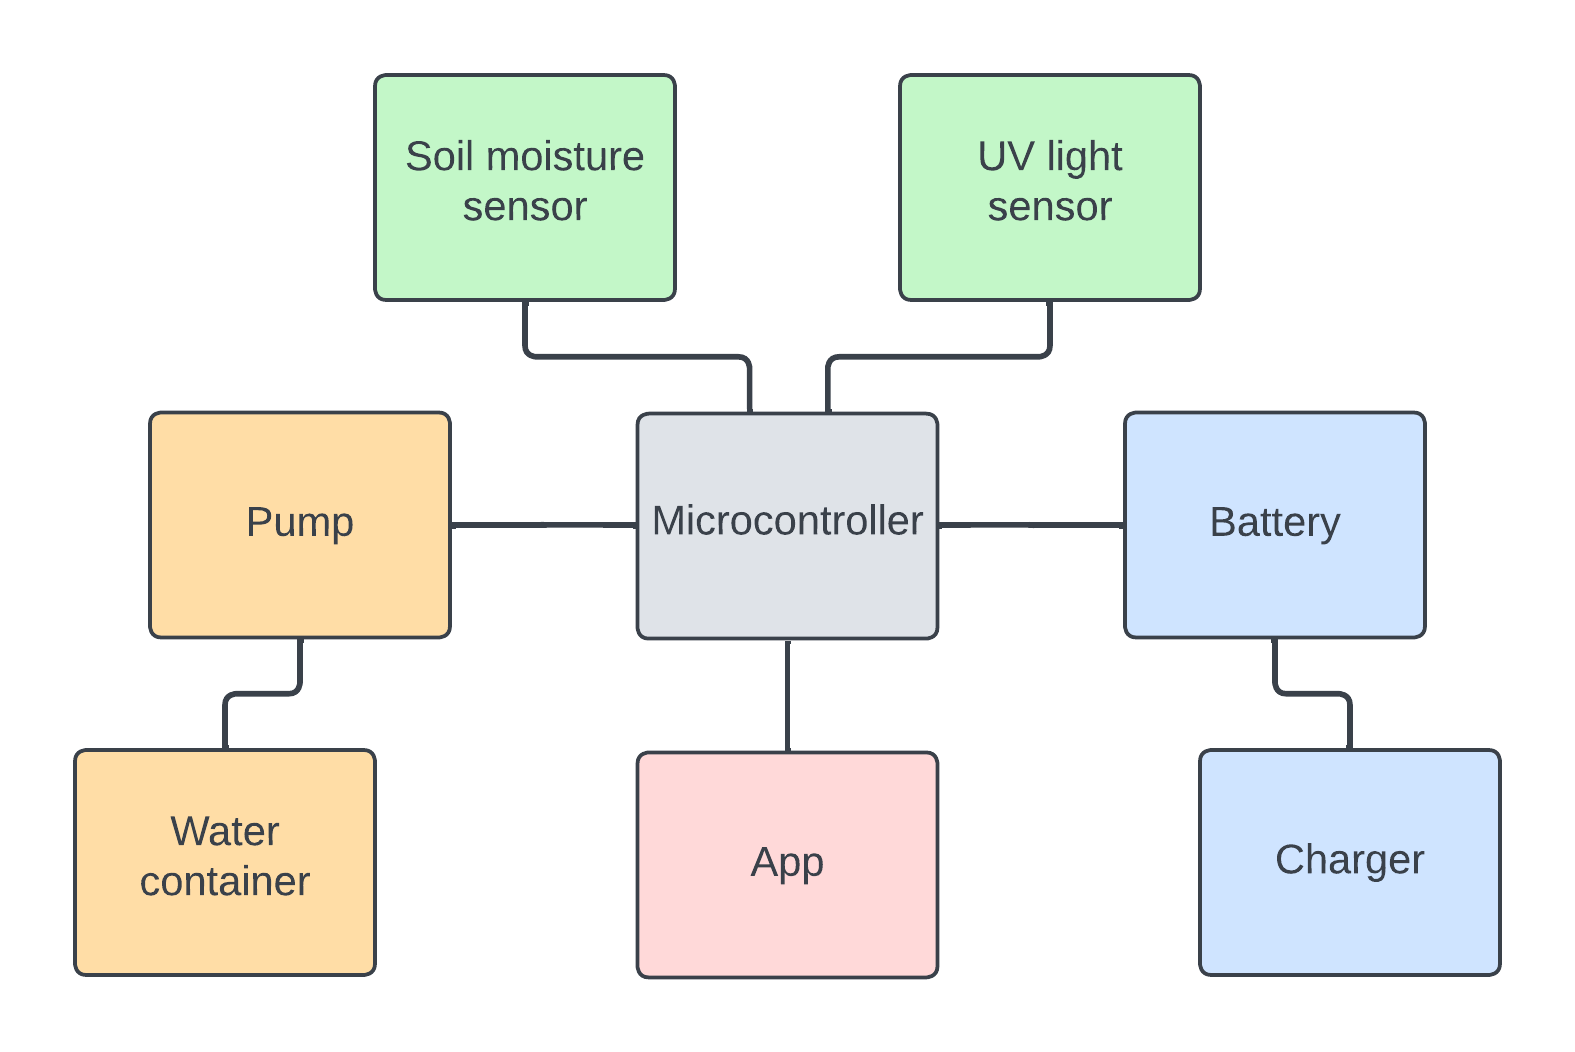
\includegraphics{design_diagram.png}
    \caption{System design overview}
    \label{fig:design_overview}
\end{figure}

This chapter describes the general requirements and design of the system. This includes the design and interactions of sub-systems as well as the selection of major components. Detailed design decisions and processes are described in chapter \ref{chap:detail_design}.

%%%%%%%%%%%%%%%%%%%%%%%%%%%%%%%%%%%%%%%%
\section{Requirements}
The project is intended for indoor use and must therefore be designed to be as small and compact as possible. \\

To function during power outages, the system will need to include a battery that can be recharged from a standard power outlet. \\

The system must be able to reliably and accurately monitor soil moisture levels and exposure to sunlight. This data must be accessible to the user and presented in a way that is easy to understand. \\

The system must be able to reliably maintain soil moisture levels by providing water automatically. The user must be able to adjust the desired soil moisture level.

%%%%%%%%%%%%%%%%%%%%%%%%%%%%%%%%%%%%%%%%
\subsection{UV light exposure and soil moisture level
measurement and logging}
The system must be able to log the average soil moisture and UV light exposure levels every minute. This data must be uploaded to be viewed on the app every 30 minutes.

%%%%%%%%%%%%%%%%%%%%%%%%%%%%%%%%%%%%%%%%
\section{System design and component selection}

Data from a soil moisture and UV light sensor will be monitored using a microcontroller. When soil moisture levels fall below a set value, a pump will turn on to water the plant until the soil reaches the target moisture level. The soil moisture, UV light exposure and watering times will be logged by the microcontroller and sent to a server. The user can use the app to view the data and set the moisture level target. The system will be powered by a battery that charges when power is available.

\begin{table}[!h]
    \centering
    \begin{tabular}{|c|c|c|c|}
        \hline
        Component & Selected & Cost & Product page \\
        \hline
        Microcontroller &  ESP32 C6 Dev Board & R 285.20 & \href{https://www.robotics.org.za/ESP32-C6-DEV}{link} \\
        UV light sensor & Wave UV Sensor Module - GUVA-S12D & R 112.70 & \href{https://www.robotics.org.za/W9537}{link} \\
        Soil moisture sensor & Capacitive Soil Moisture Sensor V1.2 & R 55.20 & \href{https://www.robotics.org.za/CAP-SW-12}{link} \\
        Pump & Digital Peristaltic Pump & R 879.95 & \href{https://www.diyelectronics.co.za/store/dfrobot/2119-digital-peristaltic-pump.html?search_query=PERISTALTIC+PUMP&results=4}{link} \\
        Battery & Li-polymer Battery HAT - 5V output & R 399.95 & \href{https://www.diyelectronics.co.za/store/hats/2726-lipo-battery-hat-5v-output.html?search_query=Li-polymer+Battery+HAT&results=14}{link}\\
        \hline
        Total & & R 1 733.00 & \\
        \hline
    \end{tabular}
    \caption{Selected components}
    \label{tab:components_selected}
\end{table}

%%%%%%%%%%%%%%%%%%%%%%%%%%%%%%%%%%%%%%%%
\subsection{Microcontroller}
Data will be sent from the microcontroller to the app using a web server. This requires the microcontroller to be connected to a WiFi network. A Bluetooth connection will be used to initially connect the microcontroller to a WiFi network.

The selection of microcontrollers with a reasonable shipping time and cost are limited. The ESP32 C6 Dev Board was selected as it has both Bluetooth and WiFi capabilities.


%%%%%%%%%%%%%%%%%%%%%%%%%%%%%%%%%%%%%%%%
\subsection{UV light and soil moisture sensing}
A capacitive soil moisture sensor will be used as they do not rust like resistive sensors do when exposed to moisture for extended time periods. This will allow the sensor to be left in the soil permanently. Both the soil moisture sensor and UV light sensor can be connected to a microcontroller without any additional circuits and output a measurement equivalent analog voltage. 

%%%%%%%%%%%%%%%%%%%%%%%%%%%%%%%%%%%%%%%%
\subsection{Automatic watering}
The pump will be powered by the battery. A driver circuit allows the pump to be controlled using the microcontroller. A peristaltic pump will be used to prevent siphoning. \\

Siphoning could also be prevented by using valves along with a small centrifugal pump, potentially resulting in a lower cost. A peristaltic pump will, however lead to a more compact system as it does not need to be submerged and can be contained within the same casing as the rest of the system. \\

The digital peristaltic pump was selected as it includes a drive circuit that takes a PWM voltage as input and requires only 5W at 5V to function.

%%%%%%%%%%%%%%%%%%%%%%%%%%%%%%%%%%%%%%%%
\subsection{App}
The app will allow the user to view the UV light exposure, soil moisture levels and watering over times. The app will also allow the user to connect the microcontroller to WiFi initially and change the target soil moisture level. Figure \ref{fig:app_flow_rough} shows the initial design of the app. 

\begin{figure}[!h]
    \centering
    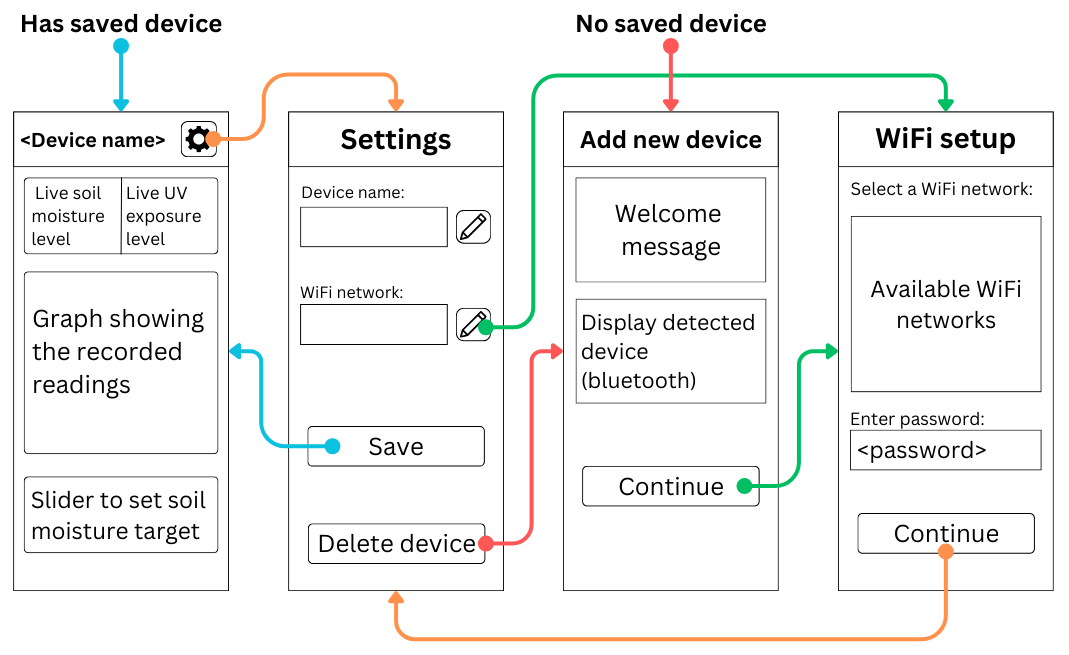
\includegraphics[width= \textwidth]{Report/general_design/fig/app_flow_rough.png}
    \caption{Initial app design}
    \label{fig:app_flow_rough}
\end{figure}



%%%%%%%%%%%%%%%%%%%%%%%%%%%%%%%%%%%%%%%%
\subsection{Battery and charging}
The battery will need to be able to power the system for at least two hours at a time to ensure the system functions during loadshedding. The battery needs to be charged whenever power is available. 
\\

Two commonly available battery types were considered: Lithium-ion and lead-acid. The following factors were compared in table \ref{tab:battery_comp}: 

\begin{itemize}
    \item \textbf{Cost:} The initial cost of the battery
    \item \textbf{Depth of discharge:} Maximum percentage of a fully charged battery that can be used before recharging
    \item \textbf{Cycle life:} The amount of charge/discharge cycles the battery can undergo without performance being affected
    \item \textbf{Power delivery:} The amount of power delivered in a charge cycle
    \item \textbf{Size:} Physical size of the battery
\end{itemize}

\begin{table}[!h]
    \centering
    \begin{tabular}{|c||c|c|}
        \hline
         &  Lead-acid & Lithium-ion \\
        \hline
        Cost & Costs less & Costs more \\
        Depth of discharge \cite{battery_10_diff} & 50\% & 80\% \\
        Cycle life \cite{battery_10_diff} & 300 - 500 cycles & 5000 cycles \\
        Power delivery \cite{battery_guide} & Starts strong but dissipates & Constant \\
        Size \cite{battery_10_diff} & Larger & Smaller \\
        \hline
    \end{tabular}
    \caption{Lithium-ion and lead-acid battery comparison}
    \label{tab:battery_comp}
\end{table}

The Li-Polymer battery HAT was chosen as it provides a 5V, 1.8A output \cite{battery_faq} and manages the charging of the included battery. The battery has a 3000mAh capacity and will be able to provide power to the system throughout loadshedding provided that the pump is not running constantly.

%%%%%%%%%%%%%%%%%%%%%%%%%%%%%%%%%%%%%%%%
\subsection{PCB}
To keep the final system as compact as possible, a PCB will be designed for the circuits.

%%%%%%%%%%%%%%%%%%%%%%%%%%%%%%%%%%%%%%%%
\subsection{Case}
The final system will be contained in a compact, durable case.
\graphicspath{{detail_design/fig/}}

\chapter{Detailed Design}
\label{chap:detail_design}

\begin{figure}[!h]
    \centering
    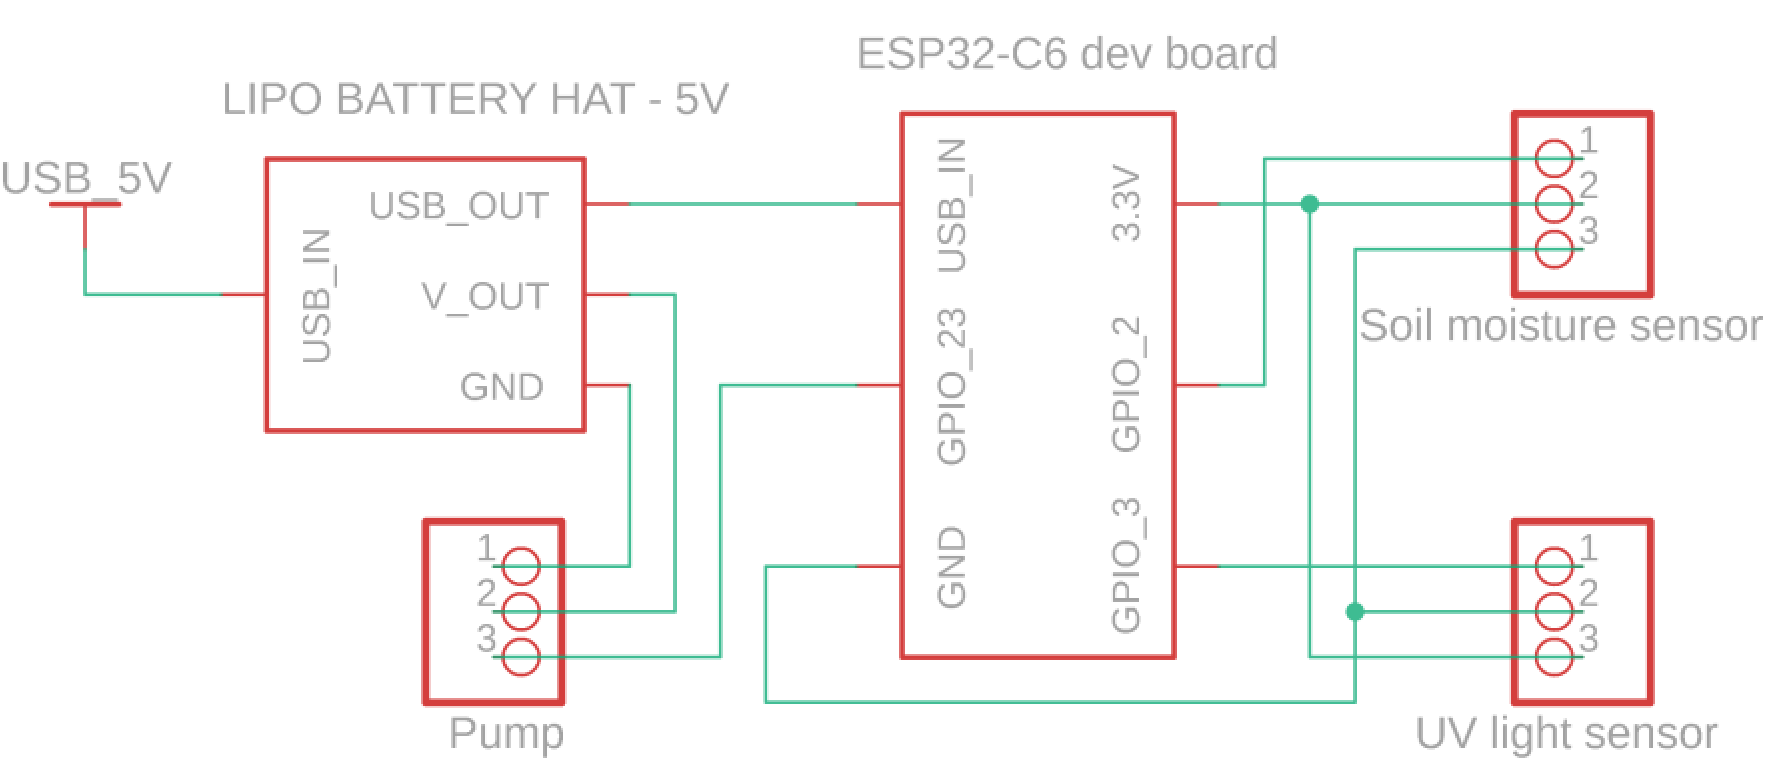
\includegraphics[width= 0.8\textwidth]{Report/detail_design/fig/detail_schematic.png}
    \caption{System schematic}
    \label{fig:detail_schematic}
\end{figure}

According to the electrical characteristics of the major components (shown in table \ref{tab:electrical_chars}), the entire system can be powered by a 5V source. The battery module will provide power to the pump and microcontroller. The sensors will be powered from the microcontroller 3.3V output. Pin 23 on the ESP32 is used to control the pump using a PWM signal, pins 2 and 3 receive the analog outputs from the soil moisture sensor and UV light sensor respectively. As shown in table \ref{tab:electrical_chars} the system will not exceed the battery module current capacity of 1.8A.

\begin{table}[!h]
\centering
\caption{Electrical characteristics of major components.}
\label{tab:electrical_chars}
    \begin{tabular}{|c||c|c||c|c|} 
        \hline
        Component & \multicolumn{2}{c||}{Input} & \multicolumn{2}{c|}{Output} \\
       %\hline
         & Voltage [V] & Current [mA] & Voltage [V] & Current [mA] \\
        \hline
        \hline
        ESP32 \cite{esp_datasheet} & 3.3 & 500 & & \\
         & 5 & & & \\
        \hline
        ESP32 pins \cite{esp_datasheet} & 0.75 * $V_{DD}$ & & 0.8 * $V_{DD}$ & 40\\
        & $V_{DD}$ + 0.3 & & & \\
        \hline
        Soil moisture sensor \cite{Moisture_sensor_datasheet} & 3.3 & $< 5$ \tablefootnote{Based off measurements} & 1.2 (high) & \\
        & 5.5 & & 2.5 (low) & \\
        \hline
        UV light sensor \cite{UV_sensor_datasheet} & 3 & 100 \tablefootnote{Maximum rating based off characteristics of similar sensors} & 0 & \\
        & 5 & & 3 & \\
        \hline
        Pump \cite{pump_datasheet} & 5 & 1000 & & \\
        \hline
        Battery module \cite{battery_datasheet} \cite{battery_faq} & 5  & 2500 & 5 & 1800 \\
        \hline
    \end{tabular}
\end{table}

%%%%%%%%%%%%%%%%%%%%%%%%%%%%%%%%%%%%%%%%
\section{Microcontroller}
Code for the microcontroller was written using the Arduino IDE, this was made possible by the esp32 (version 3.0.0-alpha3) board manager by Esspressif Systems and other contributors \cite{esp_arduino_github}. Data is stored using Firebase real-time and Firestore databases. Firebase was selected as it requires no additional device to act as a broker and allows the databases to be accessed remotely. It is also easily incorporated into Android apps using Android SDK. The Firebase Arduino client library for for Arduino devices by GitHub user mobizt (Suwatchai K.) and other contributors \cite{firebase_github} is used to interact with the databases.
\\

Three classes are used to manage external connections (Bluetooth and WiFi), data logging and uploading data. 
\begin{itemize}
    \item \textbf{DataLogger:} Calculates the average sensor readings.
    \item \textbf{ConnectionManager:} Manages the WiFi and Bluetooth connections.
    \item \textbf{DataManager:} Manages the connection to the Firebase databases, uploads logged data and retrieves device settings.
\end{itemize}

\begin{figure}[!h]
    \centering
    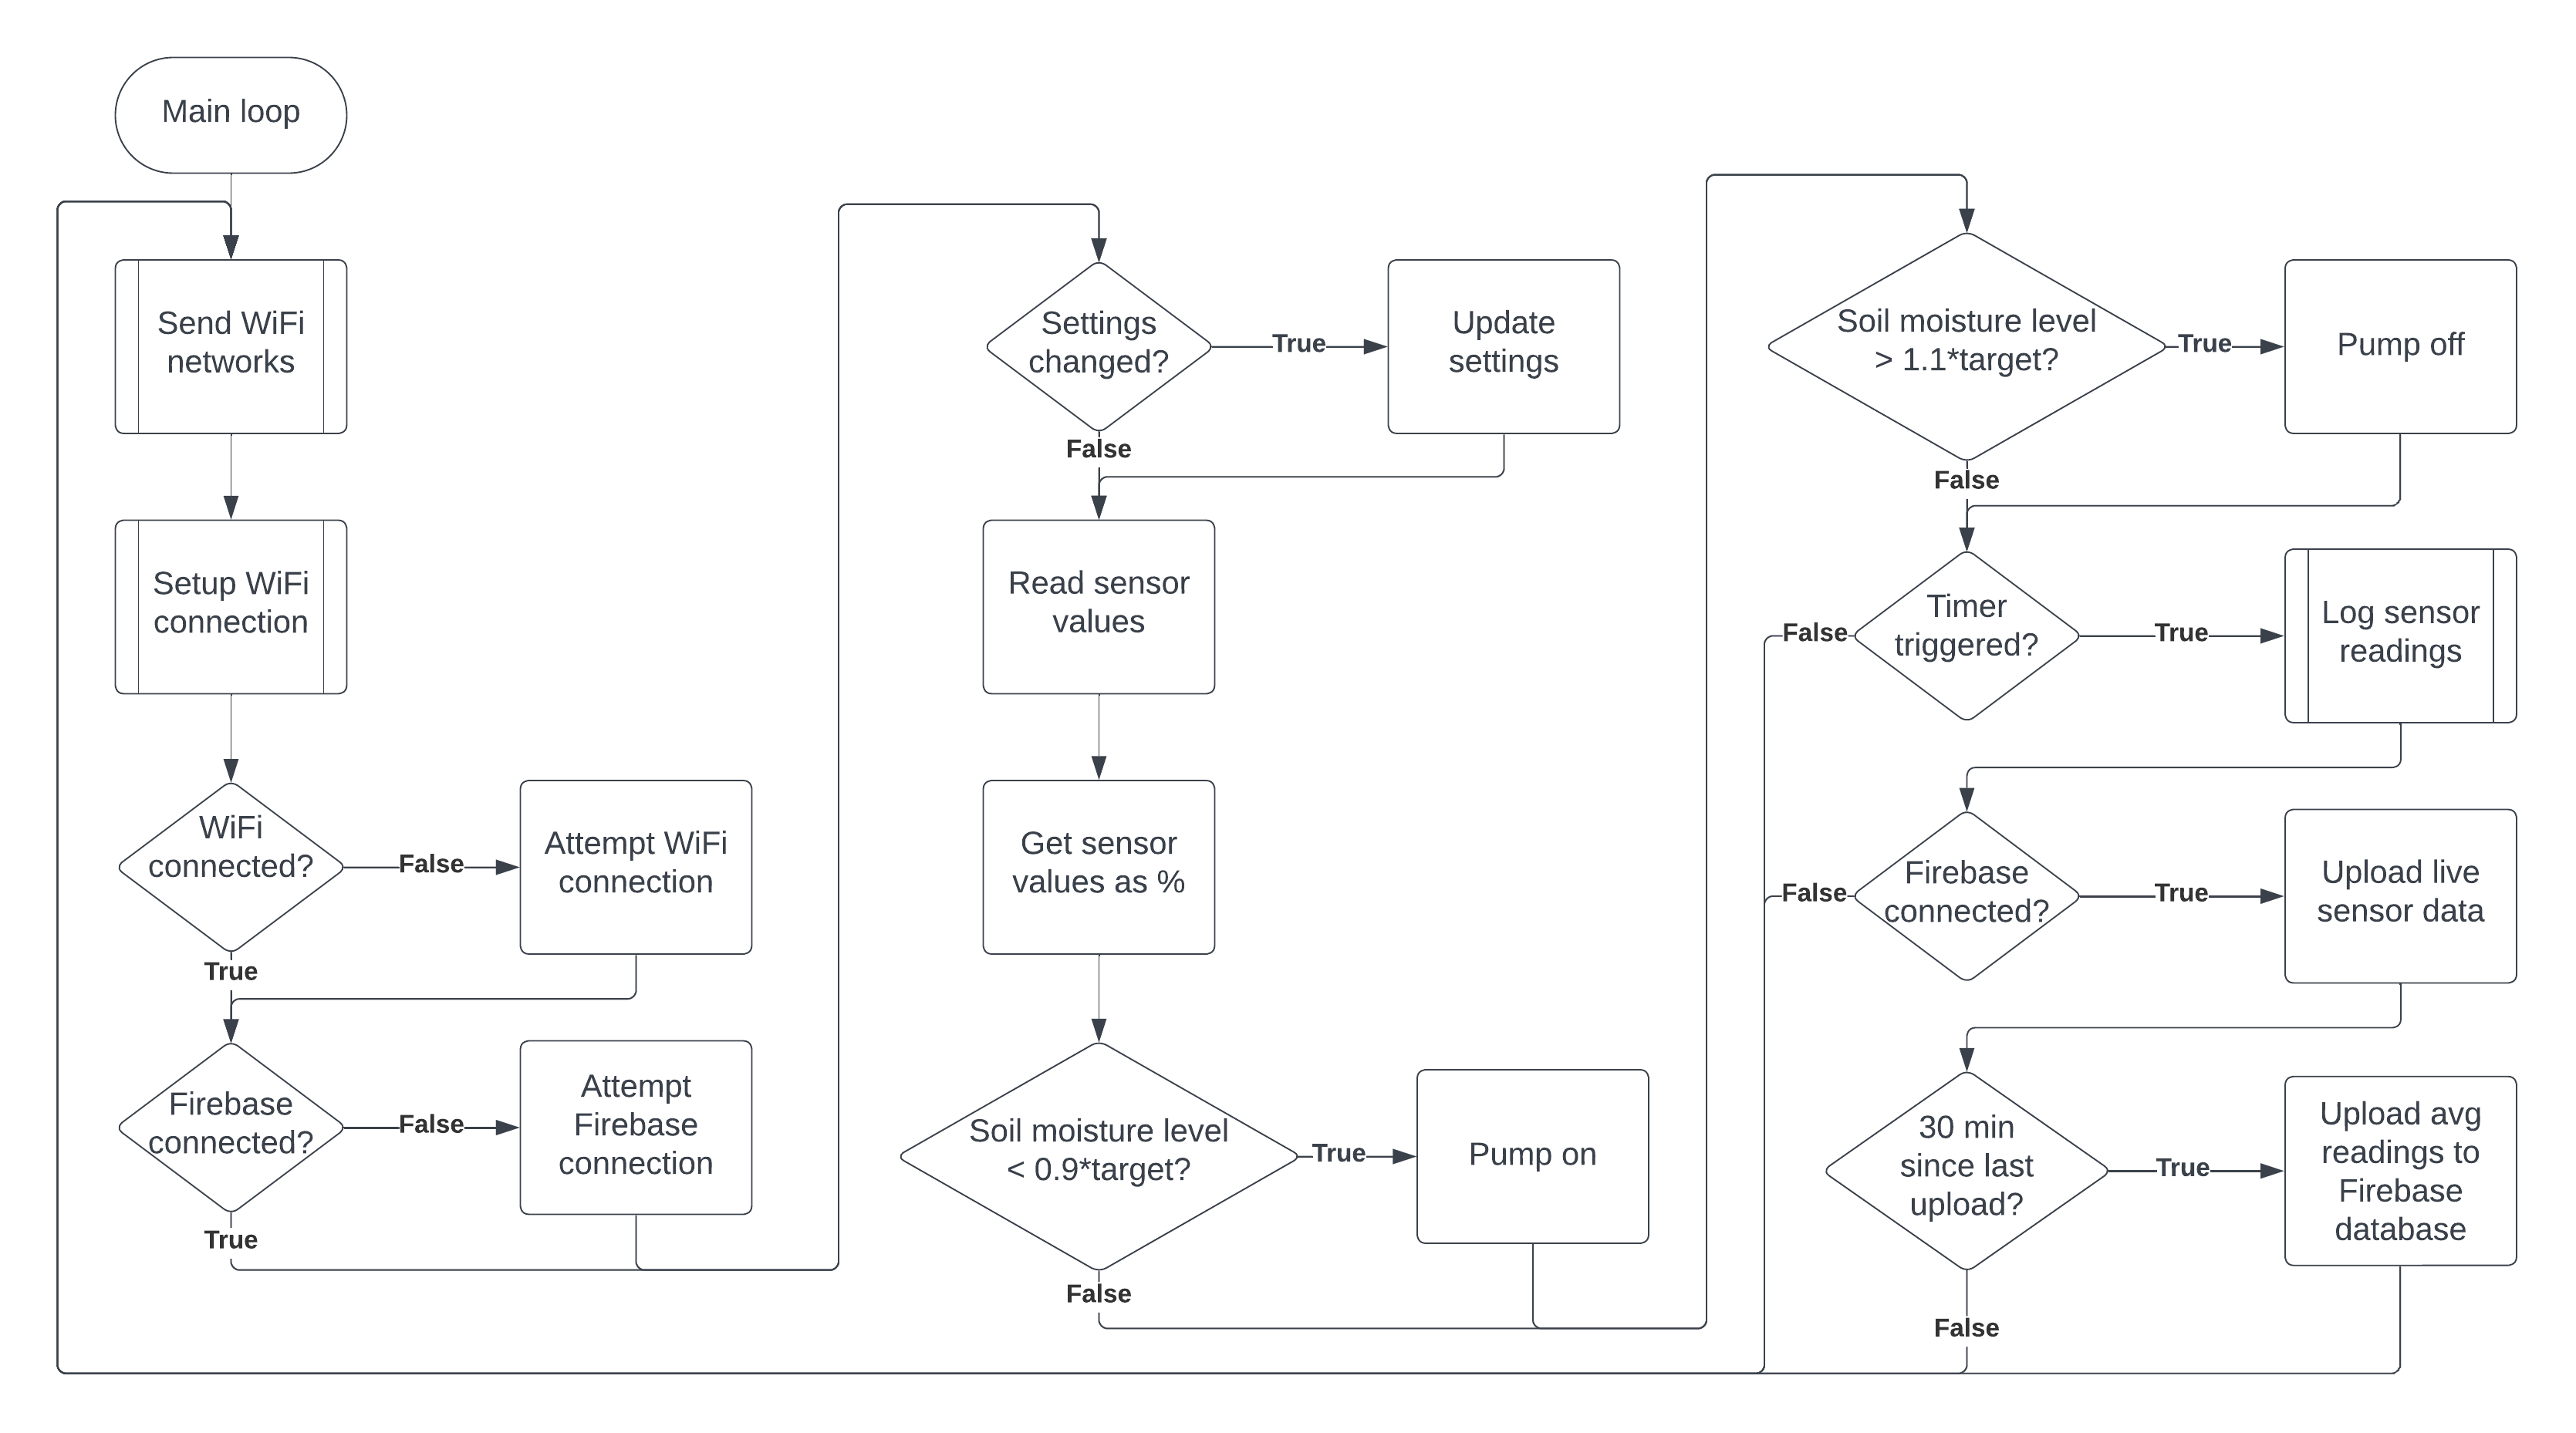
\includegraphics[width= 0.9\textwidth]{Report/detail_design/fig/main_loop_flow.png}
    \caption{Microcontroller code: main loop}
    \label{fig:main_loop_flow}
\end{figure}

The total sensor readings are updated in the main loop using a timer and interrupt that is triggered every minute. The current readings are also uploaded to the real-time database. Every 30 minutes the average sensor readings are calculated and uploaded to the Firestore database along with a timestamp.
\\
The current soil moisture levels are continuously compared to the target moisture level. The pump is turned on when the reading falls below $90\%$ of the target and is turned off once it reaches $110\%$ of the target level. Figure \ref{fig:main_loop_flow} shows a summary of the code described.

%%%%%%%%%%%%%%%%%%%%%%%%%%%%%%%%%%%%%%%%
\section{UV light exposure and soil moisture level measurement and logging}

The microcontroller uses a 5V supply to maximize the voltage output of the pins.
\\


Both the soil moisture and UV light sensors are designed to be powered by a microcontroller. Both sensors will therefore be powered using the 3.3V output pin on the ESP32. 
\\
Pins 2 and 3 (corresponding with ADC channels 2 and 3) will be used for the soil moisture and UV light sensor respectively

The default ADC measurement range of the ESP32-C6 is 0V to 1V \cite{esp_datasheet} \cite{esp_github}. The signals from the sensors must therefore be attenuated before being input to the ADC. The minimum attenuation as calculated in equation \ref{eqn:attenuation} \cite{attenuation_formula} is \(-10.37 dB\).

\begin{equation}
\label{eqn:attenuation}
\begin{split}
    Attenuation  (dB) & = 20 \cdot log_{10}\left ( \frac{V_{out}}{V_{in}} \right ) \\ 
    & = 20 \cdot log_{10}\left ( \frac{1}{3.3} \right ) \\ 
    & = -10.37 dB
\end{split}
\end{equation}

An attenuation of 11dB was used as it is the closest value provided by the ESP32 Arduino Core library \cite{esp_arduino_github} (which allows writing code for the ESP32-C6 using the Arduino IDE). 
\\
The ESP32-C6 has a 12 bit ADC \cite{esp_tech_ref}, resulting in a resolution of 4095, the sensor output ranges can be calculated using equation \ref{eqn:measured_val}. Table \ref{tab:sensor_ranges} shows the calculated measurement ranges of both sensors.

\begin{equation}
\label{eqn:measured_val}
    Measured \quad value = Resolution \cdot V_{in} \cdot 10^{Attenuation / 20}
\end{equation}

\begin{table}[!h]
    \centering
    \begin{tabular}{|c|cc|cc|}
    \hline
         & \multicolumn{2}{c||}{Soil moisture sensor} & \multicolumn{2}{c|}{UV light sensor} \\
        \hline
        Voltage & 1.2V & 2.5V & 0V & 3V \\
        Measured value & 1385 & 2885 & 0 & 3462\\
        \hline
    \end{tabular}
    \caption{Sensor value ranges}
    \label{tab:sensor_ranges}
\end{table}

%%%%%%%%%%%%%%%%%%%%%%%%%%%%%%%%%%%%%%%%
\section{Automatic watering}

%%%%%%%%%%%%%%%%%%%%%%%%%%%%%%%%%%%%%%%%
\section{App}

\begin{figure}[!h]
    \centering
    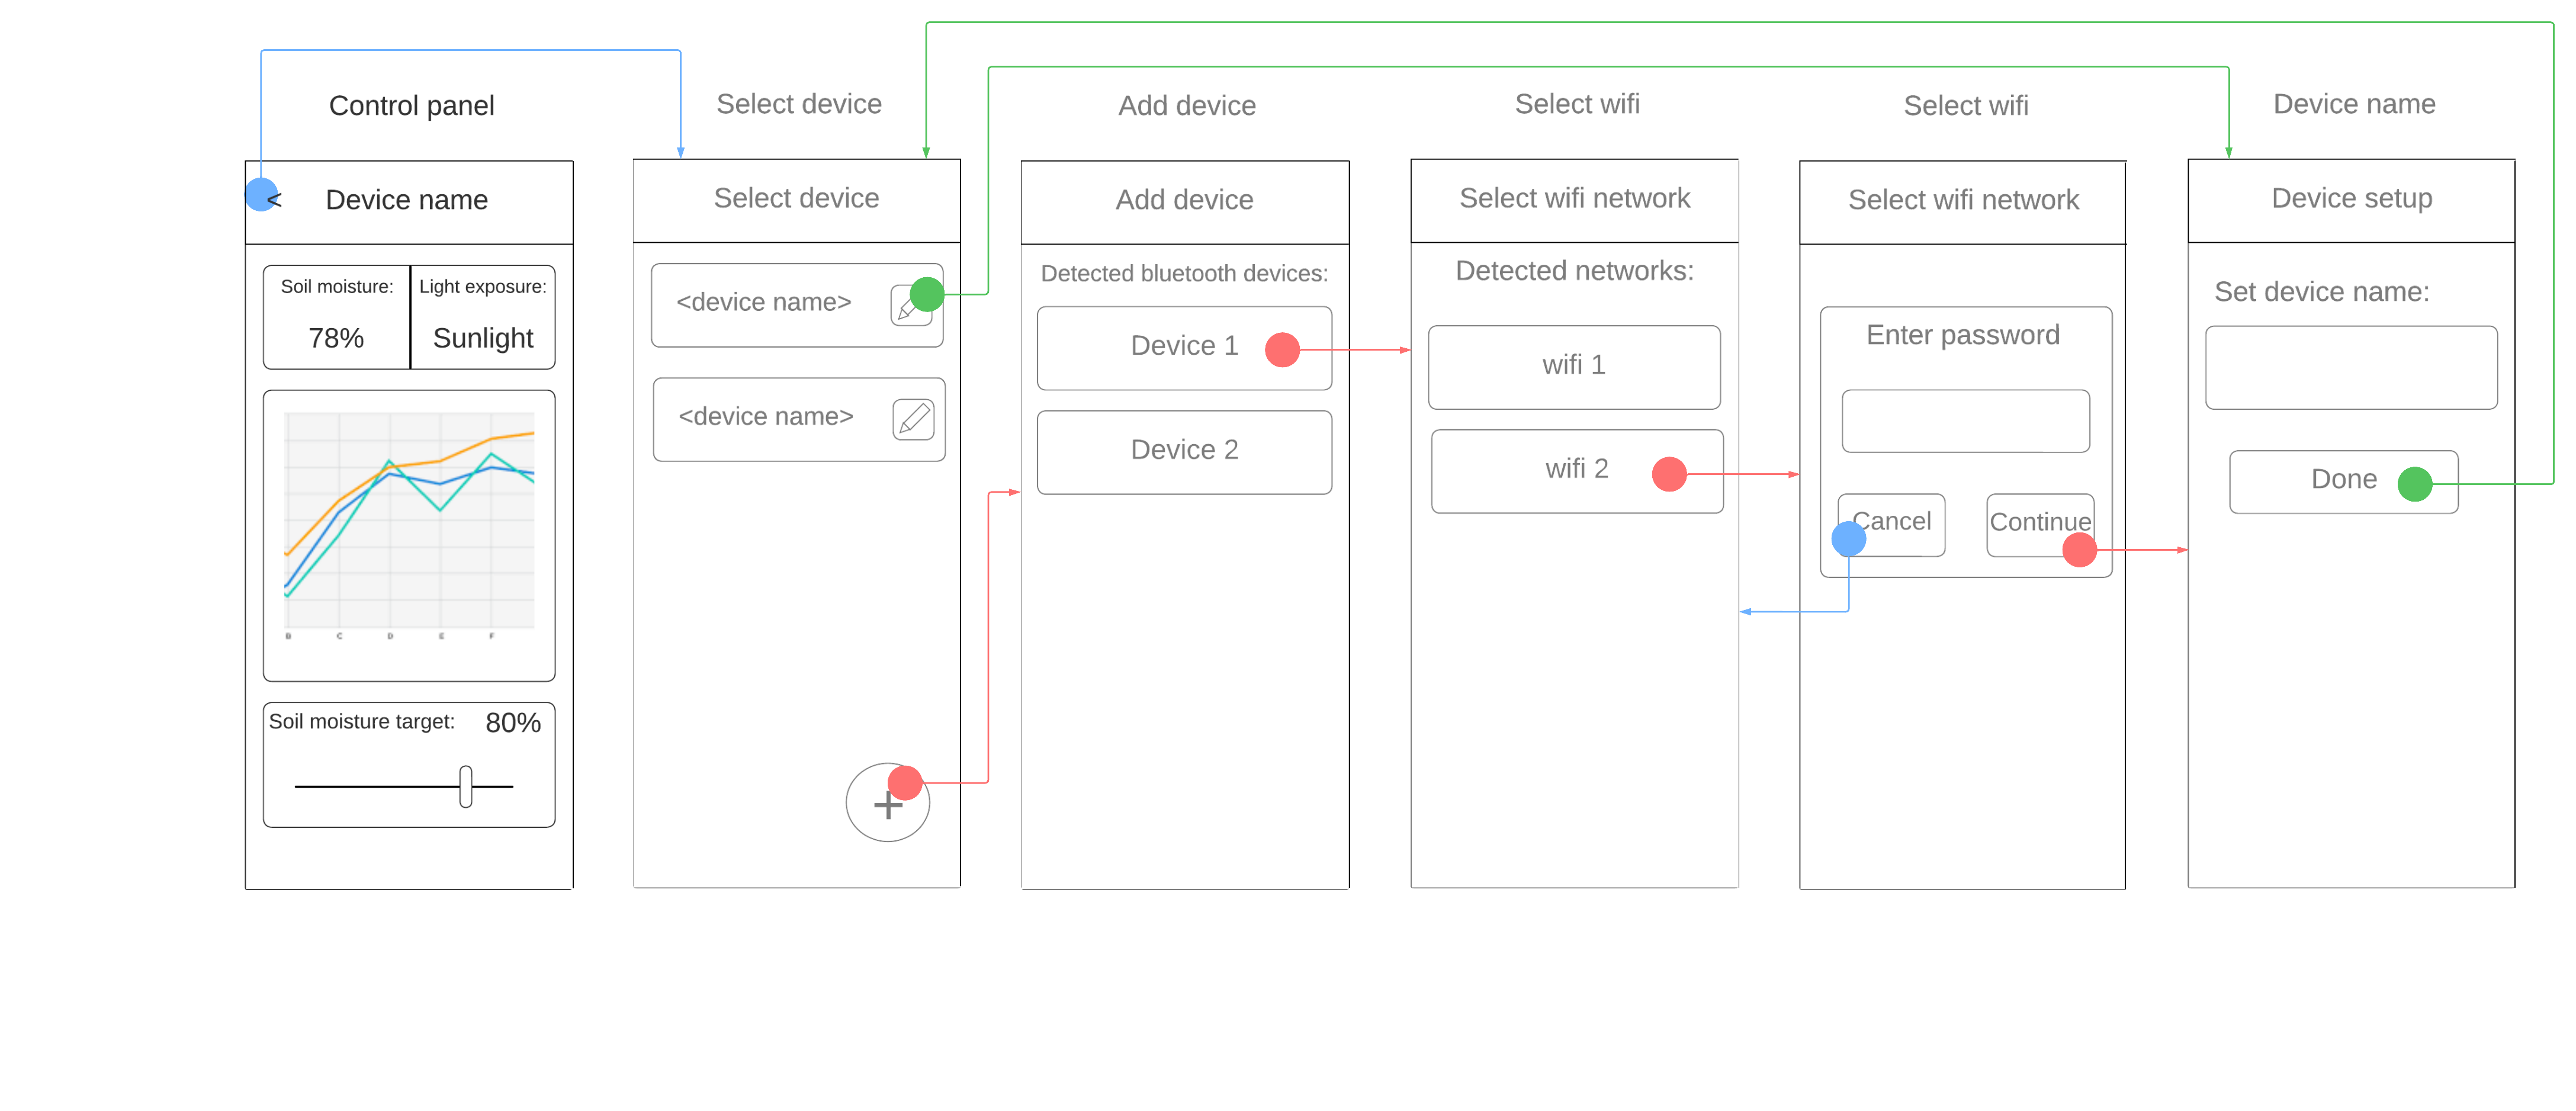
\includegraphics[width= \textwidth]{Report/detail_design/fig/app_flow.png}
    \caption{App flow}
    \label{fig:app_flow}
\end{figure}

\subsection{Connecting to WiFi}
\begin{figure}[!h]
    \centering
    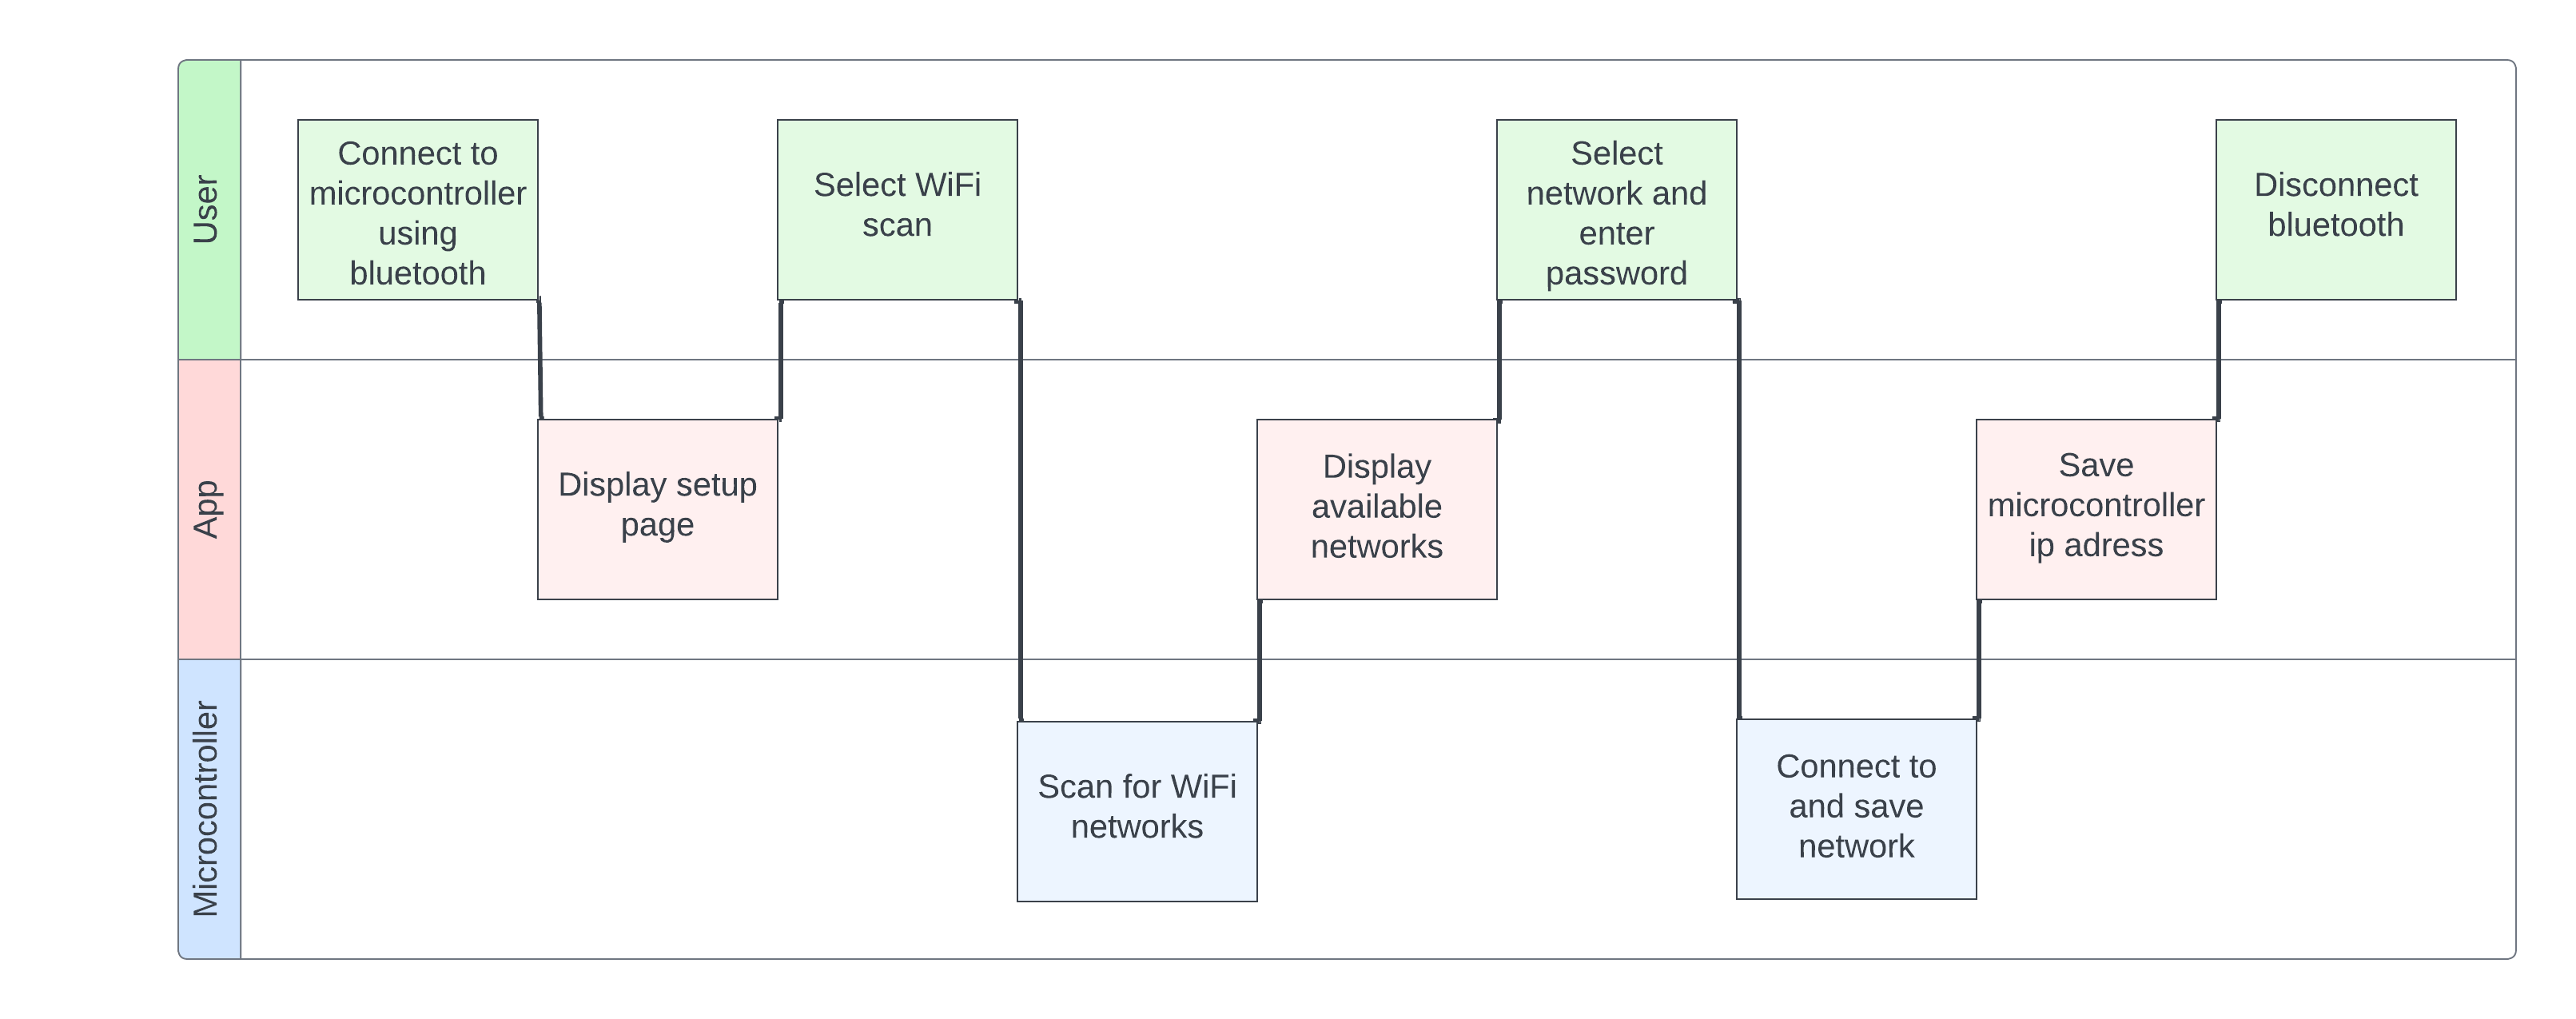
\includegraphics[width= \textwidth]{Report/detail_design/fig/wifi_connect.png}
    \caption{WiFi setup process}
    \label{fig:wifi_setup}
\end{figure}

%%%%%%%%%%%%%%%%%%%%%%%%%%%%%%%%%%%%%%%%
\section{Battery and charging}
\label{sec:battery}
\subsection{battery options}

%%%%%%%%%%%%%%%%%%%%%%%%%%%%%%%%%%%%%%%%
\section{PCB}

%%%%%%%%%%%%%%%%%%%%%%%%%%%%%%%%%%%%%%%%
\section{Case}

\graphicspath{{testing/fig/}}

\chapter{Testing and Results}
\label{chap:testing}

%%%%%%%%%%%%%%%%%%%%%%%%%%%%%%%%%%%%%%%%
\section{UV light exposure and soil moisture level measurement and
logging}

%%%%%%%%%%%
\subsection{Testing procedure}
The logging of the sensor data will be tested by placing the sensors in controlled environments to verify the readings. The sensors and microcontroller will also be placed in a planter for 24 hours to assess the data logging capability of the system.

%%%%%%%%%%%
\subsection{Results}
TO DO: fill in testing results \\
Process 24h data and make graph?

\begin{table}[!h]
    \centering
    \begin{tabular}{|c|c|c|}
        \hline
        Condition & Expected value & Measured value \\
        \hline
        Full sunlight & 100 & \\
        Partial sunlight & 20-70 & \\
        No sunlight & 0 & \\
        \hline
    \end{tabular}
    \caption{UV light sensor testing results}
    \label{tab:uv_results}
\end{table}

\begin{table}[!h]
    \centering
    \begin{tabular}{|c|c|c|}
        \hline
        Condition & Expected value & Measured value \\
        \hline
        Submerged in water & 100 & \\
        Wrapped in damp cloth & 30-80 & \\
        Dry & 0 & \\
        \hline
    \end{tabular}
    \caption{Soil moisture sensor testing results}
    \label{tab:soil_results}
\end{table}

%%%%%%%%%%%%%%%%%%%%%%%%%%%%%%%%%%%%%%%%
\section{Automatic watering}

%%%%%%%%%%%%%%%%%%%%%%%%%%%%%%%%%%%%%%%%
\section{App}

%%%%%%%%%%%%%%%%%%%%%%%%%%%%%%%%%%%%%%%%
\section{Battery and charging}

%%%%%%%%%%%%%%%%%%%%%%%%%%%%%%%%%%%%%%%%
\section{PCB}

%%%%%%%%%%%%%%%%%%%%%%%%%%%%%%%%%%%%%%%%
\section{Case}
\graphicspath{{conclusion/fig/}}

\chapter{Summary and Conclusion}
\label{chap:conclusion}


% Bibliography
\bibliography{mybib}

% End matter
\appendix
\chapter{ESP32-C6 pin assignment}
\makeatletter\@mkboth{}{Appendix}\makeatother
\label{appen:derivations_bigramseg}

\begin{table}[!h]
    \centering
    \begin{tabular}{|c|c|}
        \hline
        Pin & Function \\
        \hline
        2 & Soil moisture sensor output \\
        3 & UV light sensor output \\
        23 & PWM pump control \\
        \hline
    \end{tabular}
    \caption{Pin assignment}
    \label{tab:pin_assignment}
\end{table}

\chapter{Project Planning Schedule}
\makeatletter\@mkboth{}{Appendix}\makeatother
\label{appen:derivations_bigramseg}

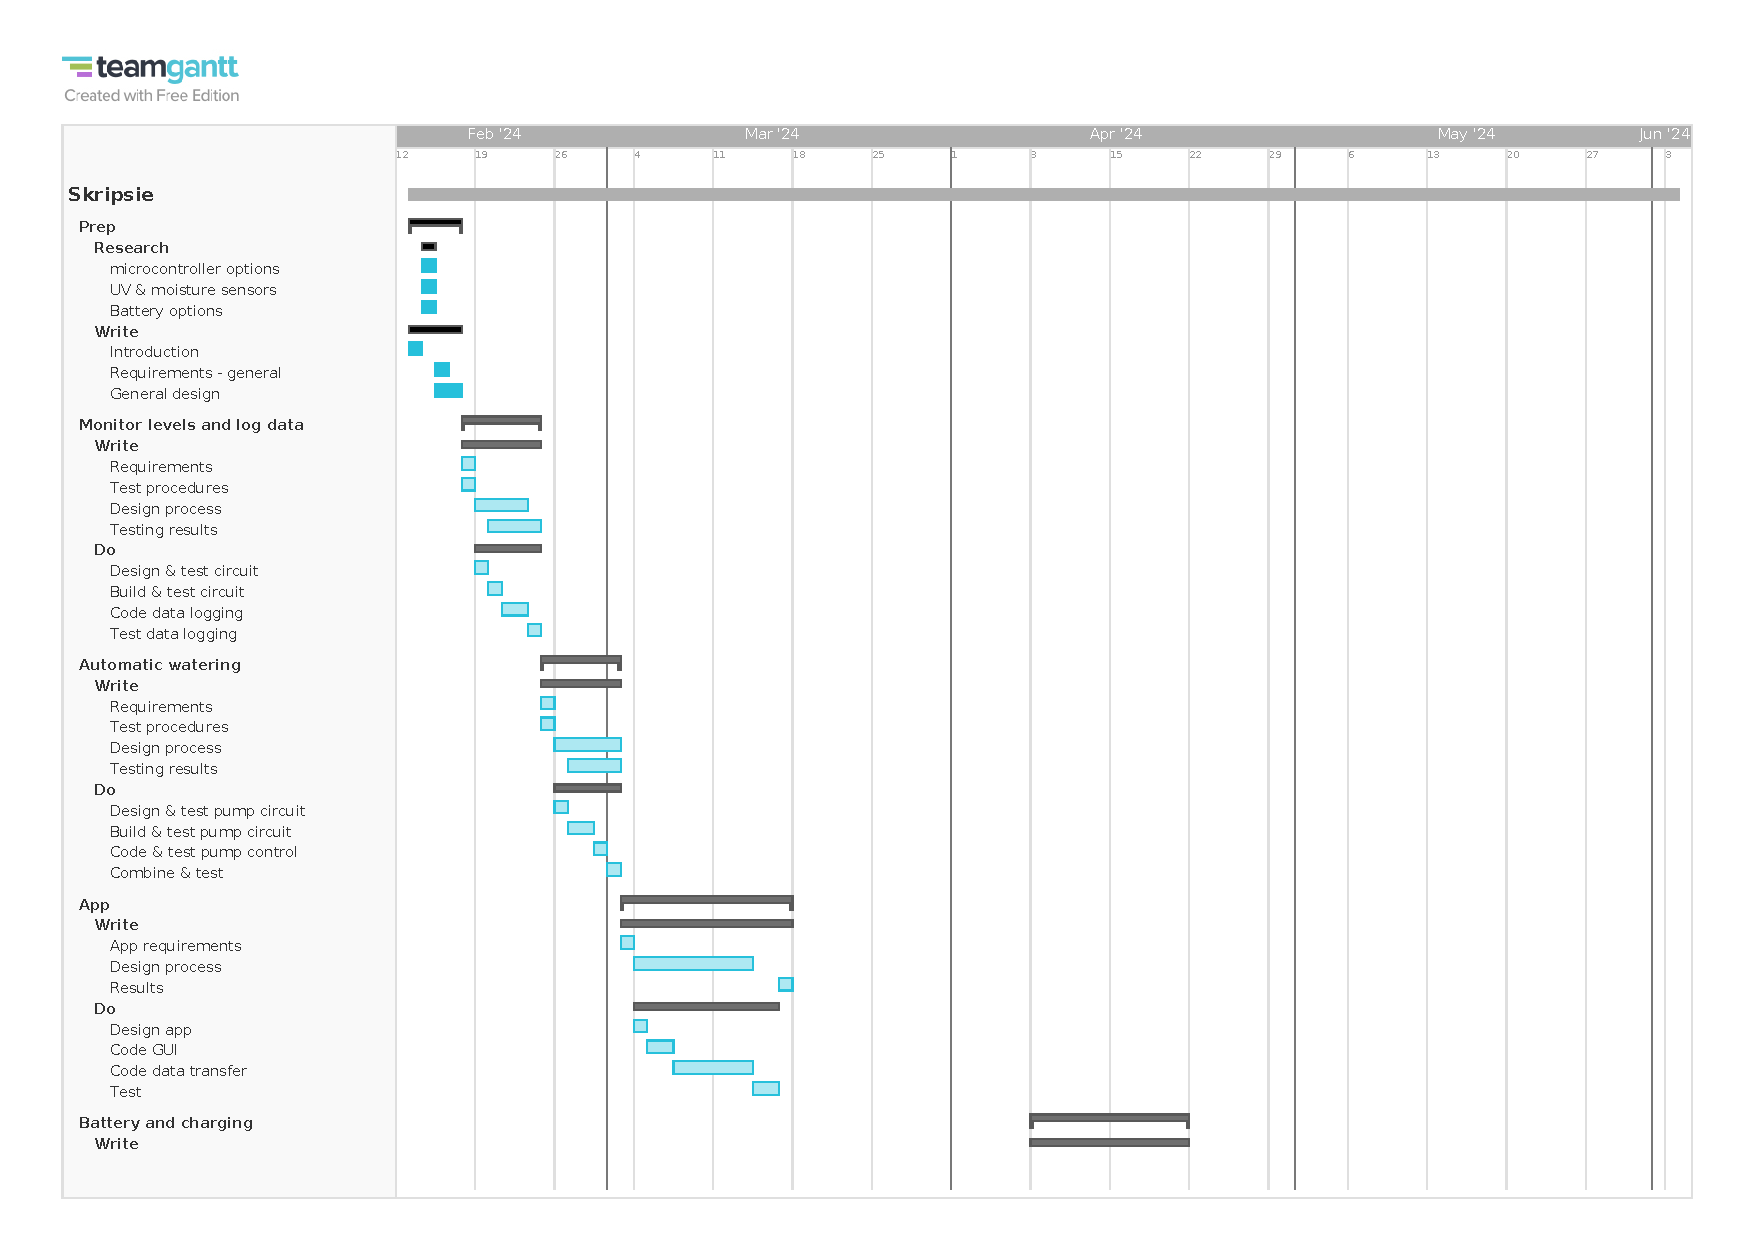
\includepdf[pages=-, landscape]{Report/appendices/project_plan.pdf}

\chapter{Outcomes Compliance}
\makeatletter\@mkboth{}{Appendix}\makeatother
\label{appen:derivations_bigramseg}

This is another appendix.



\end{document}

